\documentclass{standalone}
\usepackage{pgfplots}
\usetikzlibrary{shapes.geometric,arrows,fit,calc,positioning,matrix,backgrounds,patterns,decorations.pathreplacing}

\begin{document}
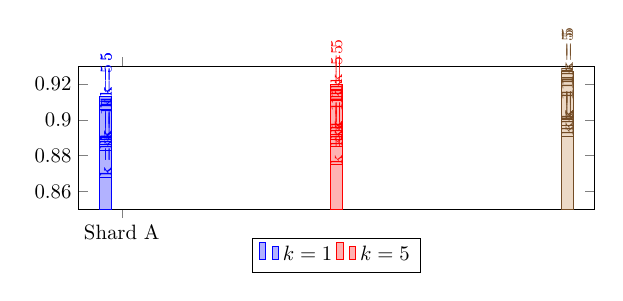
\begin{tikzpicture}[scale=0.75]
\begin{axis}[
    ybar,
    height=4cm,
    width=.85\textwidth,
    bar width=.2cm,
    ymin=0.85,ymax=0.93,
    xtick=data,
    symbolic x coords={Shard A,Shard B,Shard C},
    nodes near coords,
    point meta=explicit symbolic,
    legend style={
        at={(0.5,-0.2)},
        anchor=north,
        legend columns=-1
    },
    every node near coord/.append style={
        font=\footnotesize,
        rotate=90,
        anchor=west,
        inner sep=0pt,
        align=center
    }
]
\addplot+[] coordinates {
    % Shard A
    ({Shard A}, 0.868) [k = 1]
    ({Shard A}, 0.883) [k = 1]
    ({Shard A}, 0.888) [k = 1]
    ({Shard A}, 0.889) [k = 1]
    ({Shard A}, 0.888) [k = 1]
    ({Shard A}, 0.886) [k = 1]
    ({Shard A}, 0.868) [k = 1]
    ({Shard A}, 0.906) [k = 5]
    ({Shard A}, 0.913) [k = 5]
    ({Shard A}, 0.913) [k = 5]
};
\addplot+[] coordinates {
    % Shard B
    ({Shard B}, 0.875) [k = 1]
    ({Shard B}, 0.885) [k = 1]
    ({Shard B}, 0.889) [k = 1]
    ({Shard B}, 0.894) [k = 1]
    ({Shard B}, 0.892) [k = 1]
    ({Shard B}, 0.889) [k = 1]
    ({Shard B}, 0.894) [k = 1]
    ({Shard B}, 0.911) [k = 5]
    ({Shard B}, 0.917) [k = 5]
    ({Shard B}, 0.920) [k = 5]
};
\addplot+[] coordinates {
    % Shard C
    ({Shard C}, 0.891) [k = 1]
    ({Shard C}, 0.893) [k = 1]
    ({Shard C}, 0.900) [k = 1]
    ({Shard C}, 0.900) [k = 1]
    ({Shard C}, 0.899) [k = 1]
    ({Shard C}, 0.897) [k = 1]
    ({Shard C}, 0.900) [k = 1]
    ({Shard C}, 0.924) [k = 5]
    ({Shard C}, 0.926) [k = 5]
    ({Shard C}, 0.927) [k = 5]
};

\legend{$k = 1$,$k = 5$}
\end{axis}
\end{tikzpicture}
\end{document}